% =====================================================================
% Complete Figure Example: Skeleton C — Central Hero + 4 Panels
% =====================================================================
% USAGE: Complete compilable template, BY-CONSTRUCTION layout.
%
% ⚙ LAYOUT = BY-CONSTRUCTION (positioning + fit + node anchors): the bento
%   rhythm lives in ONE place, the 5 zones are placed relative to each
%   other, inter-zone arrows ride node anchors, each panel's internals sit
%   in a scope shift={(zone.center)}. Change content, lengthen labels, or
%   move/widen a zone and the rest REFLOWS — no coordinate bookkeeping.
%   ⚠ The x/y numbers in the LAYOUT GRID below are ORIGINAL design intent,
%   now derived — not live values. SEMANTIC constraints still hold.
%
% LAYOUT GRID (original design intent — now derived by construction):
%   Title:           y=[10.0, 11.0]   x=[0, 21]
%   LU Hyperparams:  x=[0.0,  9.5]    y=[6.0, 9.5]   teal
%   RU Benchmarks:   x=[11.0, 21.0]   y=[6.0, 9.5]   blue
%   HERO Central:    x=[0.0,  21.0]   y=[1.5, 5.5]   purple
%   LD Pipeline:     x=[0.0,  9.5]    y=[-2.5, 1.0]  gold
%   RD Metrics:      x=[11.0, 21.0]   y=[-2.5, 1.0]  green
%   Legend:          x=[0, 21]        y=[-3.5, -3.0]
%
% Sub-agent: replace titles + labels + numbers; the bento reflows by
% construction. Do not re-introduce absolute \node at (x,y) / hand rects.
% =====================================================================

\documentclass[tikz,border=15pt]{standalone}
\usepackage{xcolor,tikz,amsmath,amssymb}
\usetikzlibrary{positioning,calc,backgrounds,arrows.meta,bending,fit}

\definecolor{acaBlueLine}{HTML}{3060A8}
\definecolor{acaBlueFill}{HTML}{6890C8}
\definecolor{acaBlueBg}{HTML}{DCE6F4}
\definecolor{acaPurpleLine}{HTML}{6E3FA0}
\definecolor{acaPurpleBg}{HTML}{EDE3F6}
\definecolor{acaOrangeLine}{HTML}{D06020}
\definecolor{acaGreenLine}{HTML}{389050}
\definecolor{acaTealLine}{HTML}{1F8F8F}
\definecolor{acaTealBg}{HTML}{D3EBEB}
\definecolor{acaGoldLine}{HTML}{B08820}
\definecolor{acaGoldBg}{HTML}{F4E8CC}
\definecolor{acaGreenBg}{HTML}{DBEDDC}
\definecolor{acaGreyLine}{HTML}{606060}
\definecolor{cellLo}{HTML}{F0E8F8}
\definecolor{cellHi}{HTML}{6E3FA0}

\pgfdeclarelayer{background}
\pgfsetlayers{background,main}

% ---- single source of truth for the bento rhythm ----
\newlength{\colw}\setlength{\colw}{9.5cm}    % side-column width
\newlength{\sideh}\setlength{\sideh}{3.5cm}  % top/bottom row height
\newlength{\heroh}\setlength{\heroh}{4.0cm}  % hero band height
\def\colgap{1.5cm}                            % gap between L/R columns
\def\rowgap{0.5cm}                            % gap between rows

\tikzset{
  zone/.style={
    rectangle, rounded corners=4pt, line width=0.7pt,
    minimum width=\colw, minimum height=\sideh, anchor=north west,
    inner sep=0pt,
  },
  herozone/.style={
    rectangle, rounded corners=4pt, line width=0.7pt,
    minimum height=\heroh, anchor=north west, inner sep=0pt,
  },
  ztitle/.style={
    anchor=north, font=\small\bfseries, text=white, rounded corners=2pt,
    inner sep=3pt, inner ysep=2pt, yshift=-3pt,
  },
  base box/.style={
    rectangle, rounded corners=3pt, line width=0.5pt,
    minimum height=0.55cm, font=\scriptsize, align=center, inner sep=3pt,
  },
}

% Helper: paint a zone's background + border from its node anchors.
% #1 = node name, #2 = line color, #3 = bg color
\newcommand{\paintzone}[3]{%
  \begin{pgfonlayer}{background}
    \fill[#3!50, rounded corners=4pt]
      (#1.south west) rectangle (#1.north east);
  \end{pgfonlayer}
  \draw[#2, line width=0.7pt, rounded corners=4pt]
    (#1.south west) rectangle (#1.north east);
}

% Helper: zone title strip pinned to a zone's north anchor.
% #1 = node name, #2 = fill color, #3 = title text
\newcommand{\paintztitle}[3]{%
  \node[ztitle, fill=#2] at (#1.north) {#3};
}

\begin{document}
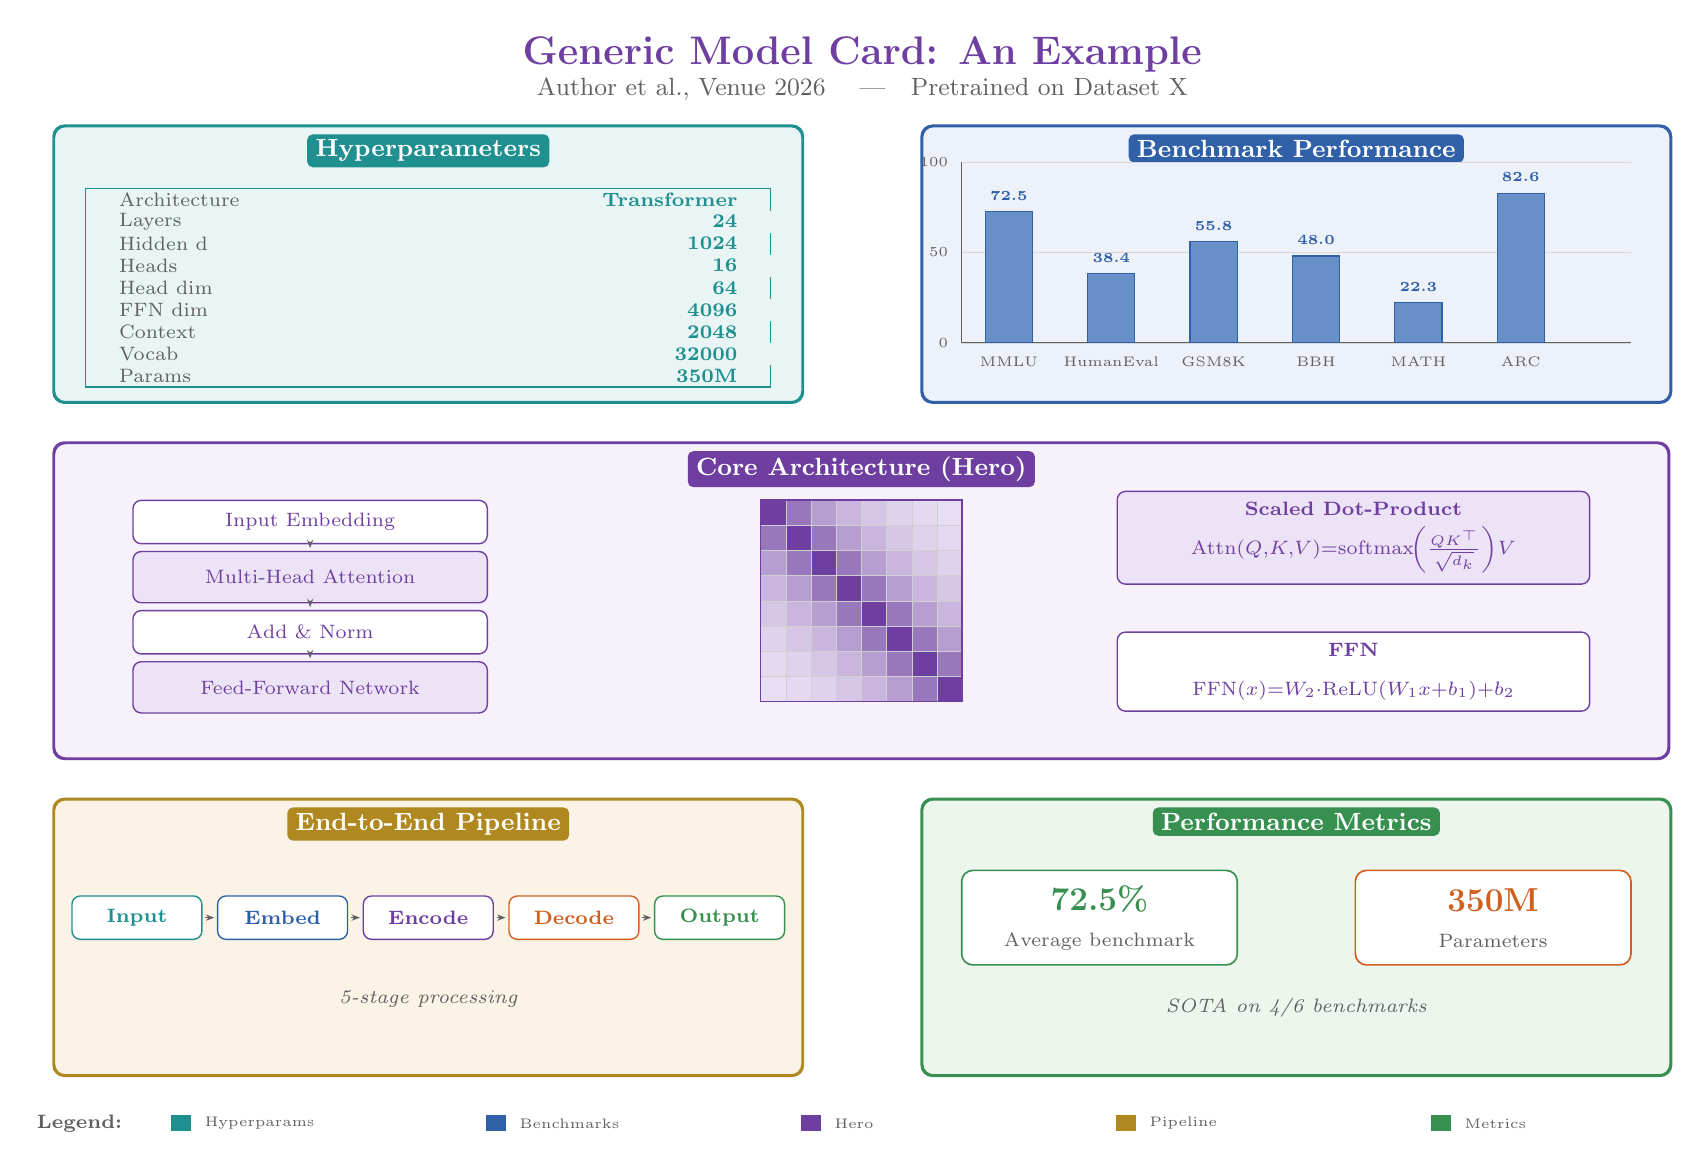
\begin{tikzpicture}

% =====================================================================
% BENTO FRAME — zones placed by construction (relative positioning)
%   row1: LU (anchored) + RU (right=of LU, gap=\colgap)
%   hero: full width, below=of LU, spanning LU.west .. RU.east
%   row3: LD (below=of hero) + RD (right=of LD)
% =====================================================================
\node[zone, draw=acaTealLine] (LU) at (0,0) {};
\node[zone, draw=acaBlueLine, right=\colgap of LU] (RU) {};

% Hero spans the full bento width; width derived from LU.west .. RU.east.
\node[herozone, draw=acaPurpleLine, below=\rowgap of LU.south west,
      anchor=north west,
      minimum width={\colw + \colgap + \colw}] (HERO) {};

\node[zone, draw=acaGoldLine, below=\rowgap of HERO.south west,
      anchor=north west] (LD) {};
\node[zone, draw=acaGreenLine, right=\colgap of LD] (RD) {};

% Zone backgrounds + borders (drawn from anchors only)
\paintzone{LU}{acaTealLine}{acaTealBg}
\paintzone{RU}{acaBlueLine}{acaBlueBg}
\paintzone{HERO}{acaPurpleLine}{acaPurpleBg}
\paintzone{LD}{acaGoldLine}{acaGoldBg}
\paintzone{RD}{acaGreenLine}{acaGreenBg}

% Zone title strips (pinned to .north of each zone)
\paintztitle{LU}{acaTealLine}{Hyperparameters}
\paintztitle{RU}{acaBlueLine}{Benchmark Performance}
\paintztitle{HERO}{acaPurpleLine}{Core Architecture (Hero)}
\paintztitle{LD}{acaGoldLine}{End-to-End Pipeline}
\paintztitle{RD}{acaGreenLine}{Performance Metrics}

% =====================================================================
% TITLE — centred over the whole bento via calc midpoint
% =====================================================================
\coordinate (bentotop) at ($(LU.north west)!0.5!(RU.north east)$);
\node[font=\Large\bfseries, color=acaPurpleLine, anchor=south]
  at ($(bentotop)+(0,0.55)$) {Generic Model Card: An Example};
\node[font=\small, color=acaGreyLine, anchor=south]
  at ($(bentotop)+(0,0.2)$)
  {Author et al., Venue 2026 \quad|\quad Pretrained on Dataset X};

% =====================================================================
% LU PANEL: Hyperparameters table — internals re-anchored to LU.center
% =====================================================================
% Local frame: origin at LU.center. Table block built in local coords so
% it travels with the zone. Original colW=8.7, rowH=0.28, 9 rows.
\begin{scope}[shift={(LU.center)}]
  \def\colW{8.7}\def\rowH{0.28}
  \def\tabdata{%
    Architecture/Transformer,%
    Layers/24,%
    Hidden d/1024,%
    Heads/16,%
    Head dim/64,%
    FFN dim/4096,%
    Context/2048,%
    Vocab/32000,%
    Params/350M%
  }
  \newcount\rowcount \rowcount=0
  \foreach \k/\v in \tabdata { \global\advance\rowcount by 1 }
  \edef\nrows{\the\rowcount}
  \pgfmathsetmacro\tabH{\nrows * \rowH}
  % Centre the table block: vertically nudge down a touch to clear title.
  \pgfmathsetmacro\xL{-\colW/2}
  \pgfmathsetmacro\yTop{\tabH/2 - 0.30}
  \draw[acaTealLine, line width=0.5pt]
    (\xL, \yTop - \tabH) rectangle (\xL + \colW, \yTop);
  \foreach [count=\idx] \k/\v in \tabdata {
    \pgfmathsetmacro\ypos{\yTop - (\idx - 1) * \rowH}
    \pgfmathsetmacro\altfill{int(mod(\idx,2))}
    \ifnum\altfill=0
      \fill[acaTealBg!50] (\xL, \ypos - \rowH) rectangle (\xL + \colW, \ypos);
    \fi
    \node[anchor=west, font=\scriptsize, color=acaGreyLine]
      at (\xL + 0.30, \ypos - \rowH/2) {\k};
    \node[anchor=east, font=\scriptsize\bfseries, color=acaTealLine]
      at (\xL + \colW - 0.30, \ypos - \rowH/2) {\v};
  }
\end{scope}

% =====================================================================
% RU PANEL: Benchmark bar chart — internals re-anchored to RU.center
% =====================================================================
\begin{scope}[shift={(RU.center)}]
  % Local chart frame: width \bcW, height \bcH, baseline at \yBase.
  \def\bcW{8.5}\def\bcH{2.3}
  \pgfmathsetmacro\xBase{-\bcW/2}
  \pgfmathsetmacro\yBase{-1.0}
  \draw[acaGreyLine, line width=0.4pt] (\xBase, \yBase) -- (\xBase + \bcW, \yBase);
  \draw[acaGreyLine, line width=0.4pt] (\xBase, \yBase) -- (\xBase, \yBase + \bcH);
  \foreach \pct in {0, 50, 100} {
    \pgfmathsetmacro\ypos{\yBase + \bcH * \pct / 100}
    \draw[acaGreyLine!25, line width=0.2pt]
      (\xBase, \ypos) -- (\xBase + \bcW, \ypos);
    \node[anchor=east, font=\tiny, color=acaGreyLine]
      at (\xBase - 0.05, \ypos) {\pct};
  }
  % 6 bars: spacing 1.3, width 0.6, first bar centre at \xBase + 0.6.
  \foreach \i/\name/\val in {1/MMLU/72.5, 2/HumanEval/38.4, 3/GSM8K/55.8,
                            4/BBH/48.0, 5/MATH/22.3, 6/ARC/82.6} {
    \pgfmathsetmacro\cx{\xBase + 0.6 + (\i - 1) * 1.3}
    \pgfmathsetmacro\bh{\bcH * \val / 100}
    \pgfmathsetmacro\bxL{\cx - 0.3}
    \pgfmathsetmacro\bxR{\cx + 0.3}
    \pgfmathsetmacro\btop{\yBase + \bh}
    \fill[acaBlueFill] (\bxL, \yBase) rectangle (\bxR, \btop);
    \draw[acaBlueLine, line width=0.4pt] (\bxL, \yBase) rectangle (\bxR, \btop);
    \node[font=\tiny\bfseries, color=acaBlueLine, anchor=south]
      at (\cx, \btop + 0.02) {\val};
    \node[font=\tiny, color=acaGreyLine, anchor=north]
      at (\cx, \yBase - 0.05) {\name};
  }
\end{scope}

% =====================================================================
% HERO PANEL: 3 internal sub-zones — all re-anchored to HERO.center
% =====================================================================
% Hero internal layout (local coords, origin at HERO.center):
%   Left:   sub-module stack
%   Middle: attention heatmap (centred at local x=0)
%   Right:  2 formula boxes
\begin{scope}[shift={(HERO.center)}]
  % --- Left: sub-module stack (4 boxes), centred near local x=-7 ---
  \def\lx{-7.0}
  \node[base box, fill=white, draw=acaPurpleLine, text=acaPurpleLine,
        minimum width=4.5cm] (h1) at (\lx, 1.0) {Input Embedding};
  \node[base box, fill=acaPurpleBg, draw=acaPurpleLine, text=acaPurpleLine,
        minimum width=4.5cm, minimum height=0.65cm] (h2) at (\lx, 0.3)
    {Multi-Head Attention};
  \node[base box, fill=white, draw=acaPurpleLine, text=acaPurpleLine,
        minimum width=4.5cm] (h3) at (\lx, -0.4) {Add \& Norm};
  \node[base box, fill=acaPurpleBg, draw=acaPurpleLine, text=acaPurpleLine,
        minimum width=4.5cm, minimum height=0.65cm] (h4) at (\lx, -1.1)
    {Feed-Forward Network};
  \foreach \a/\b in {h1/h2, h2/h3, h3/h4} {
    \draw[-{Stealth[length=3pt]}, line width=0.4pt, color=acaGreyLine,
          shorten >=1pt, shorten <=1pt]
      (\a.south) -- (\b.north);
  }

  % --- Middle: attention heatmap, centred at local x=0 ---
  \def\cs{0.32}\def\N{8}
  \pgfmathsetmacro\xH{-\N*\cs/2}
  \pgfmathsetmacro\yH{\N*\cs/2}
  \foreach \i in {1,...,\N} {
    \foreach \j in {1,...,\N} {
      \pgfmathsetmacro\val{exp(-abs(\i-\j)/2.5)*100}
      \pgfmathsetmacro\val{int(\val)}
      \pgfmathsetmacro\cx{\xH + (\j - 0.5) * \cs}
      \pgfmathsetmacro\cy{\yH - (\i - 0.5) * \cs}
      \fill[cellHi!\val!cellLo]
        (\cx - \cs/2, \cy - \cs/2) rectangle (\cx + \cs/2, \cy + \cs/2);
    }
  }
  \draw[step=\cs cm, acaGreyLine!30, line width=0.15pt]
    (\xH, \yH) grid (\xH + \N*\cs, \yH - \N*\cs);
  \draw[acaPurpleLine, line width=0.5pt]
    (\xH, \yH) rectangle (\xH + \N*\cs, \yH - \N*\cs);

  % --- Right: 2 formula boxes, centred near local x=6.25 ---
  \def\rx{6.25}
  \node[rectangle, rounded corners=3pt, fill=acaPurpleBg,
        draw=acaPurpleLine, line width=0.5pt, inner sep=4pt,
        align=center, text=acaPurpleLine, minimum width=6.0cm]
    (form1) at (\rx, 0.8)
    {{\scriptsize\bfseries Scaled Dot-Product}\\[2pt]
     $\scriptstyle\text{Attn}(Q,K,V) = \text{softmax}\!\left(\frac{QK^\top}{\sqrt{d_k}}\right) V$};
  \node[rectangle, rounded corners=3pt, fill=white,
        draw=acaPurpleLine, line width=0.5pt, inner sep=4pt,
        align=center, text=acaPurpleLine, minimum width=6.0cm]
    (form2) at (\rx, -0.9)
    {{\scriptsize\bfseries FFN}\\[2pt]
     $\scriptstyle\text{FFN}(x) = W_2 \cdot \text{ReLU}(W_1 x + b_1) + b_2$};
\end{scope}

% =====================================================================
% LD PANEL: Pipeline — internals re-anchored to LD.center
% =====================================================================
\begin{scope}[shift={(LD.center)}]
  % 5 boxes centred horizontally about local x=0. Pitch 1.85, width 1.65.
  % First-box offset so the 5-box block is symmetric: -(5-1)/2 * pitch.
  \foreach \i/\name/\col in {1/Input/acaTealLine, 2/Embed/acaBlueLine,
                            3/Encode/acaPurpleLine, 4/Decode/acaOrangeLine,
                            5/Output/acaGreenLine} {
    \pgfmathsetmacro\cx{(\i - 3) * 1.85}
    \node[rectangle, rounded corners=3pt, fill=white, draw=\col,
          line width=0.5pt, font=\scriptsize\bfseries, text=\col,
          minimum width=1.65cm, minimum height=0.55cm]
      (pip\i) at (\cx, 0.25) {\name};
  }
  \foreach \a/\b in {1/2, 2/3, 3/4, 4/5} {
    \draw[-{Stealth[length=3pt]}, line width=0.4pt, color=acaGreyLine,
          shorten >=1pt, shorten <=1pt]
      (pip\a.east) -- (pip\b.west);
  }
  \node[font=\scriptsize\itshape, color=acaGreyLine, anchor=north]
    at (0, -0.55) {5-stage processing};
\end{scope}

% =====================================================================
% RD PANEL: Metric cards — internals re-anchored to RD.center
% =====================================================================
\begin{scope}[shift={(RD.center)}]
  \node[draw=acaGreenLine, fill=white, rounded corners=4pt,
        line width=0.6pt, minimum width=3.5cm, minimum height=1.2cm,
        align=center, inner sep=4pt]
    at (-2.5, 0.25)
    {{\large\bfseries\color{acaGreenLine} 72.5\%}\\[1pt]
     {\scriptsize\color{acaGreyLine} Average benchmark}};
  \node[draw=acaOrangeLine, fill=white, rounded corners=4pt,
        line width=0.6pt, minimum width=3.5cm, minimum height=1.2cm,
        align=center, inner sep=4pt]
    at (2.5, 0.25)
    {{\large\bfseries\color{acaOrangeLine} 350M}\\[1pt]
     {\scriptsize\color{acaGreyLine} Parameters}};
  \node[font=\scriptsize\itshape, color=acaGreyLine, anchor=north]
    at (0, -0.65) {SOTA on 4/6 benchmarks};
\end{scope}

% =====================================================================
% LEGEND strip — anchored below the bottom row (tracks LD/RD)
% =====================================================================
\coordinate (legL) at ($(LD.south west)+(1.0,-0.6)$);
\node[font=\scriptsize\bfseries, color=acaGreyLine, anchor=east]
  at (legL) {Legend:};
\foreach \i/\col/\lab in {%
  1/acaTealLine/Hyperparams,%
  2/acaBlueLine/Benchmarks,%
  3/acaPurpleLine/Hero,%
  4/acaGoldLine/Pipeline,%
  5/acaGreenLine/Metrics%
} {
  \coordinate (lsw) at ($(legL)+(0.5,0)+(\i*4.0-4.0,0)$);
  \fill[\col] ($(lsw)+(0,-0.1)$) rectangle ($(lsw)+(0.25,0.1)$);
  \node[anchor=west, font=\tiny, color=acaGreyLine]
    at ($(lsw)+(0.3,0)$) {\lab};
}

\end{tikzpicture}
\end{document}
